\documentclass[conference]{IEEEtran}
\IEEEoverridecommandlockouts
% The preceding line is only needed to identify funding in the first footnote. If that is unneeded, please comment it out.
\usepackage{cite}
\usepackage{amsmath,amssymb,amsfonts}
\usepackage{algorithmic}
\usepackage{graphicx}
\usepackage{textcomp}
\usepackage{xcolor}
\usepackage{siunitx}
\def\BibTeX{{\rm B\kern-.05em{\sc i\kern-.025em b}\kern-.08em
    T\kern-.1667em\lower.7ex\hbox{E}\kern-.125emX}}
\begin{document}

\title{A Digital-Analog Converter Design Based on a Five-Transistor OTA\\
}

\author{\IEEEauthorblockN{ Huang Ruiqi}
\IEEEauthorblockA{\textit{Shanghaitech University} \\
huangrq2024@shanghaitech.edu.cn 2024531064}

}

\maketitle

\begin{abstract}
This work presents a 3-bit R-2R ladder digital-to-analog converter (DAC) implemented in a 180 nm CMOS process and driven by a custom five-transistor operational transconductance amplifier (OTA). 
The OTA provides an open-loop gain of \SI{41.5}{\deci\bel} and a unity-gain bandwidth of \SI{765.8098}{\mega\hertz} under a differential input, supporting the DAC's current-to-voltage conversion. 
Circuit-level simulations show that the output spans \SIrange{0.902}{1.425}{\volt} with a maximum differential nonlinearity of \SI{0.31}{LSB} and integral nonlinearity of \SI{0.33}{LSB}, ensuring monotonic code transitions without missing codes. 
These results demonstrate that a compact 5Transistor OTA combined with a minimal R-2R network can achieve low-power and high-linearity conversion suitable for area- and energy-constrained mixed-signal systems.
\end{abstract}

\begin{IEEEkeywords}
Digital-to-Analog Converter (DAC), R-2R Ladder, Operational Transconductance Amplifier (OTA), CMOS Circuit Design
\end{IEEEkeywords}

\section{Introduction}
This project implements a low-power, compact 3-bit R-2R ladder DAC in a \SI{180}{\nano\meter} CMOS process, driven by a custom five-transistor OTA that provides differential input voltage to single-ended output voltage conversion. 
The design has two main parts: (1) the 5-Transistor OTA, which uses an NMOS current mirror front end and a PMOS active-load differential pair to achieve high gain with minimal devices; and (2) the R-2R ladder DAC, which employs transmission-gate bit switches and precision resistor ratios to realize binary-weighted currents and full-scale output. 
The remainder of this paper is organized as follows: Section II details the 5Transistor OTA architecture, sizing, and verification; Section III covers device characterization and bias optimization; Section IV presents the 3-bit DAC principle, ladder theory, current division, and transfer function derivation; 
Section V provides the circuit topology, implementation choices, and simulation results including DNL/INL metrics; Section VI analyzes non-idealities (resistor mismatch, switch $R_{on}$, OTA limitations); Section VII concludes the work and outlines future improvements.
\section{Five-Transistor OTA}

\subsection{The system architecture}

\begin{figure}[htbp]
\centerline{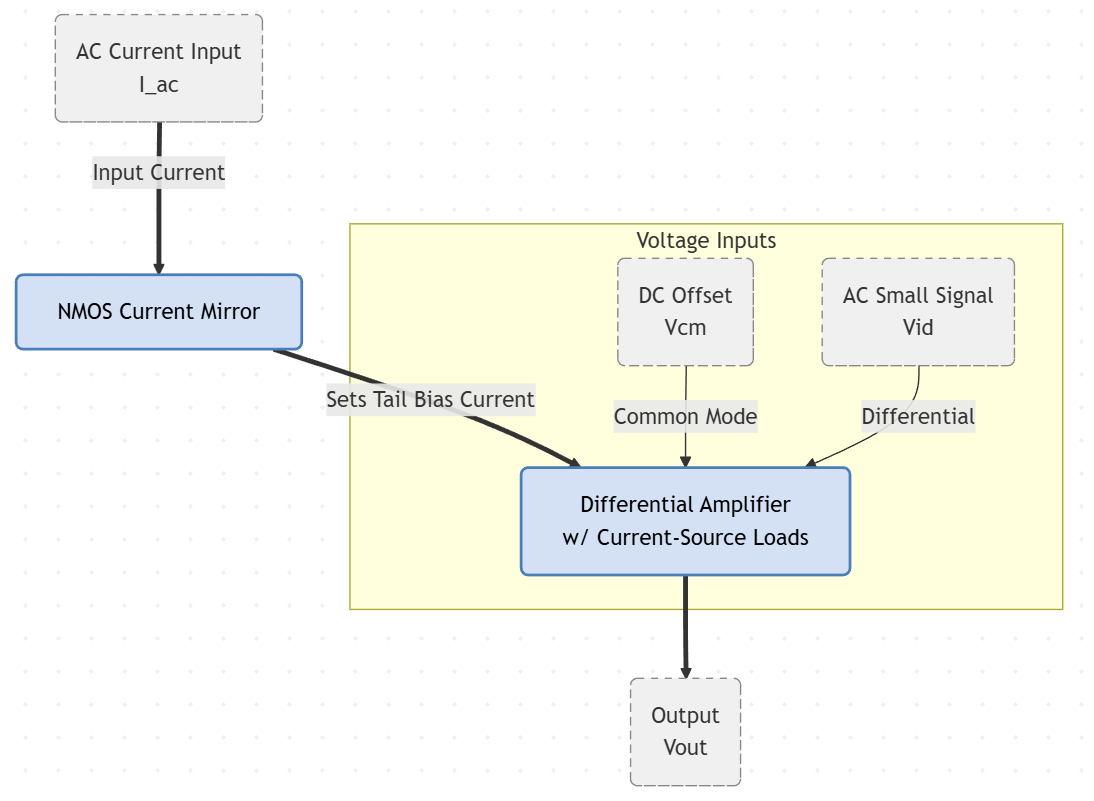
\includegraphics[width=0.45\textwidth]{Schematic.png}}
\caption{5-Transistor OTA Schematic}
\label{fig:ota_schematic}
\end{figure}

This circuit converts a differential voltage input into a single-ended voltage output through the use of an NMOS Current Mirror and a Differential Amplifier with Current-Source Loads. Next, we will analyze these two functional modules respectively.

\subsubsection{NMOS Current Mirror}

The NMOS Current Mirror serves as the input stage of the OTA, responsible for converting the input offset current signal into a Differential Amplifier with Current-Source Loads. 
The ratio of W and L of the differential pair is a key parameter that determines the input voltage of the Current-Source Loads.

\subsubsection{Differential Amplifier with Current-Source Loads}
This block serves as the core gain stage of the OTA and is composed of two distinct sub-circuits, each performing specific functions:

\begin{itemize}
    \item \textbf{NMOS Differential Input Pair:} 
    Comprising two transistors, acting as the transconductance ($G_m$) stage. 
    Its primary function is to sense the differential input voltage ($V_{id} = V_{in+} - V_{in-}$) and convert it into differential signal currents. 
    It achieves this by steering the fixed tail current between the two branches based on the input voltage difference.

    \item \textbf{PMOS Current Mirror Load (Active Load):} 
    Comprising 2 PMOS, this sub-circuit functions as an active load and performs two critical tasks:
    \begin{enumerate}
        \item \textbf{Differential-to-Single-Ended Conversion:} It mirrors the signal current from the left branch (input side) to the right branch (output side), 
        allowing the signal currents from both the M1 and M2 paths to combine constructively at the single output node.
        \item \textbf{High Voltage Gain:} By providing a high small-signal output resistance ($r_{o}$) instead of a low-impedance passive resistor, 
        it maximizes the total output impedance at the drain node, thereby generating a significantly higher voltage gain.
    \end{enumerate}
\end{itemize}

\subsection{Circuit Design and Sizing}

\section{Device Characterization and Sizing}

To determine the appropriate transistor dimensions for the proposed OTA, we analyzed the characteristics of the \texttt{TSMC180nmP} (PMOS) and \texttt{TSMC180nmN} (NMOS) models. The objective was to determine the specific Aspect Ratio ($W/L$) required to sustain a target load current of $10 \mu A$ under the circuit's operating conditions.

\subsection{Threshold Voltage Extraction}
First, a DC Sweep simulation was performed on both diode-connected NMOS and PMOS devices. The simulation results indicate that the absolute threshold voltage for both devices is approximately:
\[
|V_{th}| \approx 0.47 V
\]

\subsection{Transistor Sizing for Target Bias Current}
To simulate the operating conditions within the OTA, we biased both transistors in the saturation region with the following parameters:
\[
V_{DS} = V_{GS} = 0.6 V
\]
With the overdrive voltage fixed, we swept the dimensions to match the target drain current ($I_D$) of $10 \mu A$. The results indicated that for both devices, the channel width ($W$) must be significantly larger than the channel length ($L$). The optimized ratios are:

\begin{itemize}
    \item \textbf{NMOS Sizing:} To achieve $I_D = 10 \mu A$, the required aspect ratio is $W/L =\frac{3\mu m }{1\mu m}=3 $ (or $W:L = 3:1$).
    \item \textbf{PMOS Sizing:} To achieve the same current, a larger width is required due to the lower hole mobility. The required aspect ratio is $W/L = \frac{12\mu m}{1\mu m}=12$ (or $W:L = 12:1$).
\end{itemize}

\subsection{Simulation Verification}

\begin{figure}[htbp]
\centerline{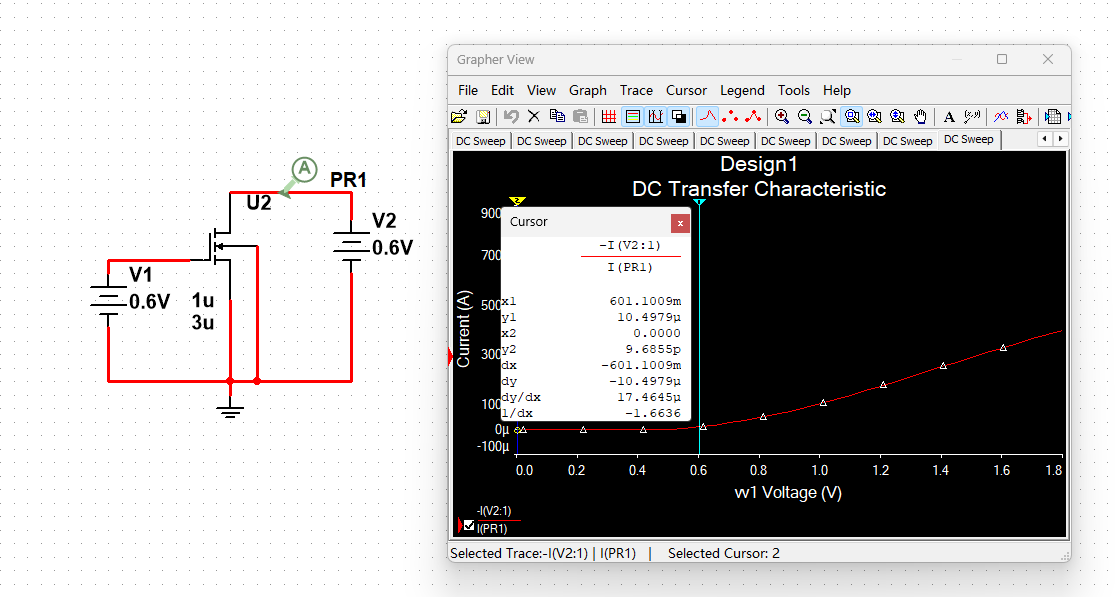
\includegraphics[width=0.35\textwidth]{NMOS.png}}
\caption{Single NMOS Test Circuit}
\label{fig:nmos_iv_curve}
\end{figure}


\begin{figure}[htbp]
\centerline{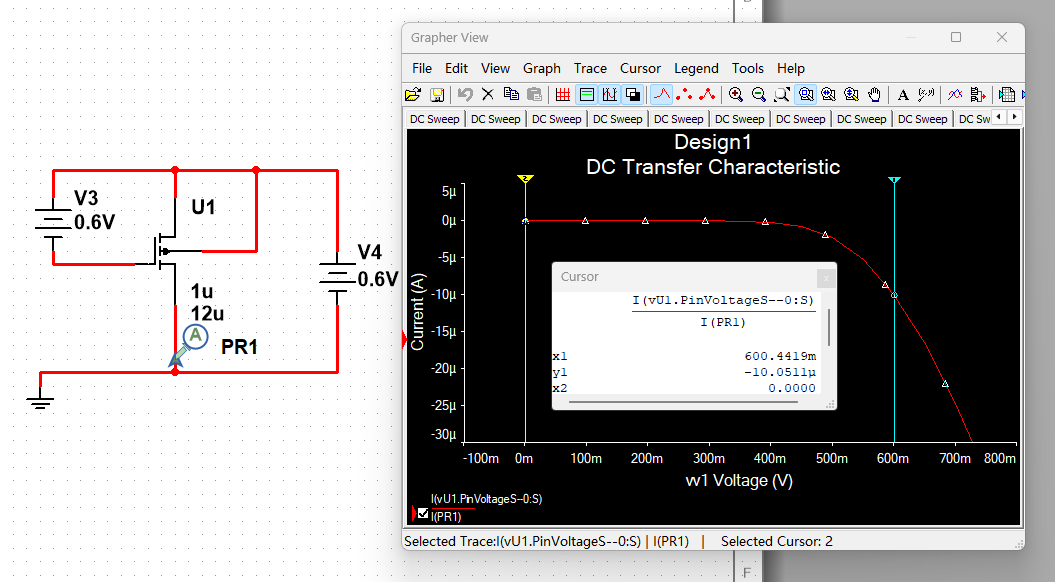
\includegraphics[width=0.35\textwidth]{PMOS.png}}
\caption{Single PMOS Test Circuit}
\label{fig:pmos_iv_curve}
\end{figure}

After the verification, we build the open loop circuit in MULTISIM. In this circuit, to apply a 20 $\mu A$ bias current to the differential pair, 
the NMOS current mirror is designed with one side having a $W/L$ of 3 and the other side having a $W/L$ of 6. And the other transistors' $W/L$ are set as the previous section.

\begin{figure}[htbp]
\centerline{
\includegraphics[width=0.35\textwidth]{Open_Loop.png}}
\caption{Open Loop Circuit of 5 transistor OTA }
\label{fig:open_loop_circuit}
\end{figure}

At the gates of the NMOS differential pair, an offset voltage consisting of a common-mode voltage of $1.2\ \mathrm{V}$and a very small AC signalis applied. 
To guarantee that all transistors operate within the saturation region, the devices comprising the PMOS current mirror and the differential pair are biased with absolute gate-source 
and drain-source voltages of $0.6\,\mathrm{V}$ (i.e., $|V_{GS}| \approx |V_{DS}| \approx 0.6\,\mathrm{V}$).\\

Also,in Fig.\ref{fig:open_loop_circuit},the total current of the circuit measured by probe 4,the total current is $29.9\mu A \leq 60 \mu A$. Requirement matched.

Then we verify the open-loop gain and Unity Gain Bandwidth by AC sweep analysis shown in Figure \ref{fig:ugb}.
\begin{figure}[htbp]
\centerline{
\includegraphics[width=0.35\textwidth]{UGB.png}}
\caption{open-loop gain and Unity Gain Bandwidth check}
\label{fig:ugb}
\end{figure}
In Figure \ref{fig:ugb}, we obtain an open-loop gain of \SI{41.5}{\deci\bel} and a unity-gain frequency of \SI{765.8098}{\mega\hertz}. Check matched the target specifications.

After that, we build the close loop circuit in MULTISIM by adding a 2pF capacitor as the load of the previous open loop circuit shown in Fig.\ref{fig:close_loop_circuit}.
\begin{figure}[htbp]
\centerline{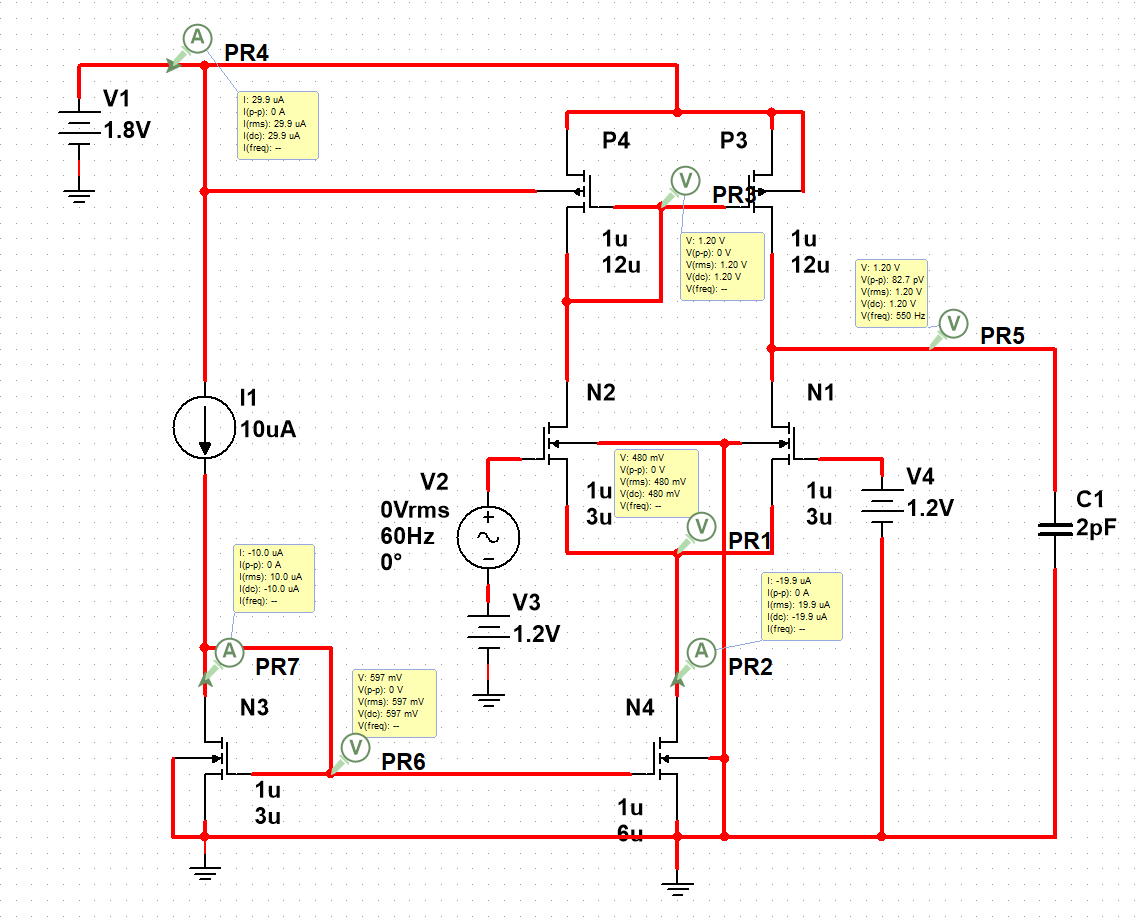
\includegraphics[width=0.35\textwidth]{Close Loop.png}}
\caption{Close-Loop Circuit and transistor operating points}
\label{fig:close_loop_circuit}
\end{figure}

Fig.\ref{fig:close_loop_0.9V} and Fig.\ref{fig:close_loop_1.5V}is the working conditions of the close loop circuit when the input common-mode voltage is \SI{0.9}{\volt} and \SI{1.5}{\volt} respectively.
The working conditions are good and all transistors are in the saturation region under the condition of a common mode offset between \SI{0.9}{\volt} and \SI{1.5}{\volt}.

\begin{figure}[htbp]
\centerline{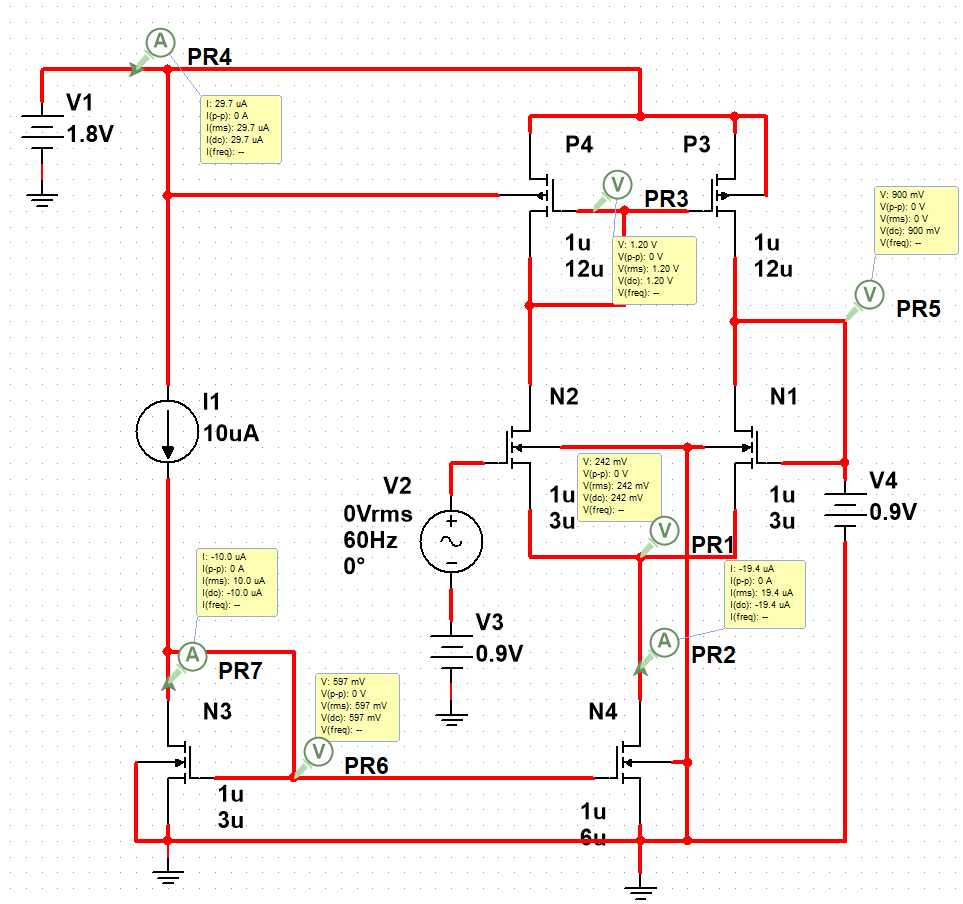
\includegraphics[width=0.35\textwidth]{0.9.png}}
\caption{$V_{CM}= 0.9V$for Closed Loop circuit}
\label{fig:close_loop_0.9V}
\end{figure}

\begin{figure}[htbp]
\centerline{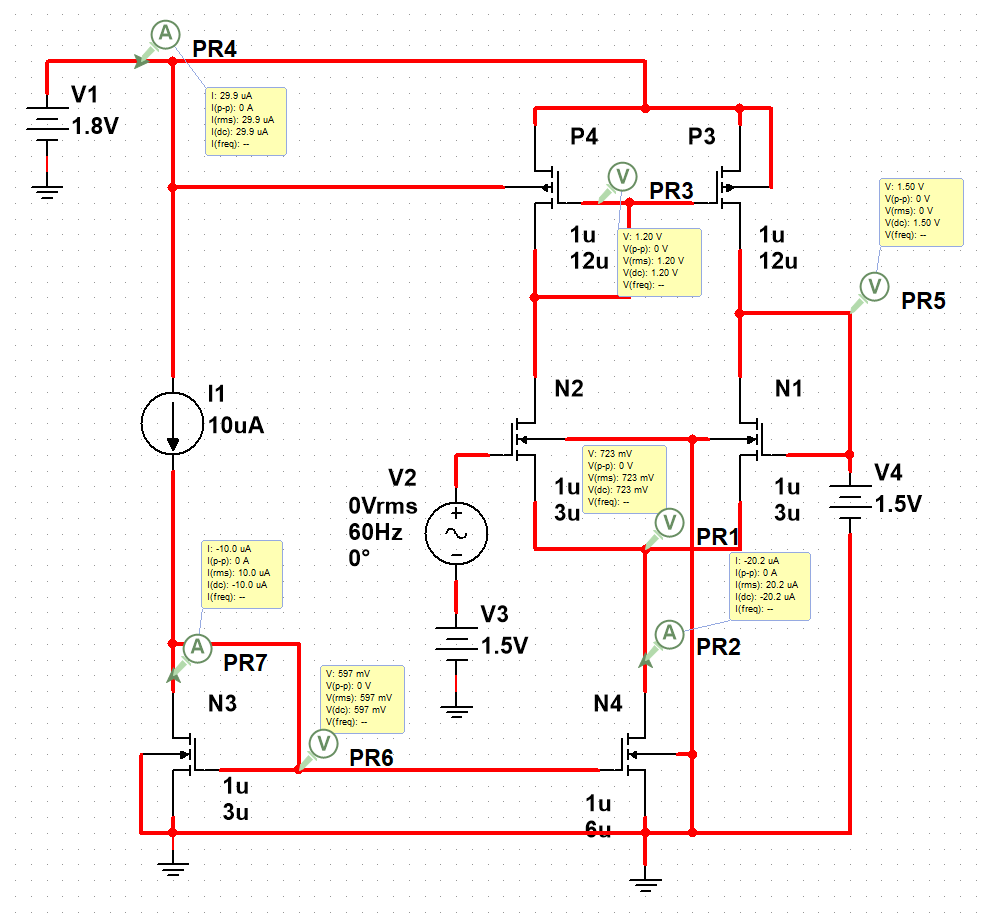
\includegraphics[width=0.35\textwidth]{1.5.png}}
\caption{$V_{CM}= 1.5V$ for Closed Loop circuit}
\label{fig:close_loop_1.5V}
\end{figure}



%============================================================================================3 Bit DAC=====================================================================================
\section{3 BIT DAC}
\subsection{Principle}
The 3-bit DAC is a circuit that convets three-bit binary digital signal input into an analog signal output. in the circuit our digital signal input is realized by a buffer formed
 by a NMOS, which from left to right represents b1, b2, b3 where b1 represents MSB, b3 represents LSB. Here we use a make a 4-bit R-2R based DAC with the following sign convention:
 the output analog voltage signal is $V_{out}$, the input reference voltage is $V_{ref}$, and the input digital signal Bin=b1b2b3, representing the concatenation of b1, b2, b3.
\[
V_{\text{out}} = V_{\text{ref}} \times B_{\text{in}} = V_{\text{ref}} \left( b_1 2^{-1} + b_2 2^{-2} + \cdots + b_N 2^{-N} \right)
\]

\begin{figure}[htbp]
\centerline{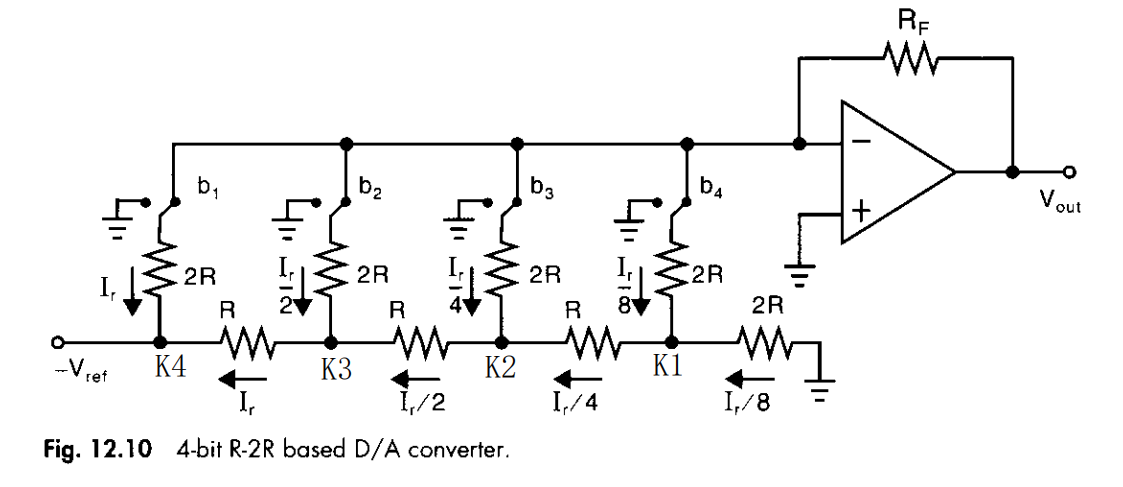
\includegraphics[width=0.5\textwidth]{4 Bit.png}}
\caption{4-bit R-2R based D/A converter.}
\label{fig:dac_diagram}
\end{figure}

\subsubsection{Theoretical Proof of R-2R Ladder Functionality}
Let $R_{eq, k}$ be the equivalent resistance looking to the right from node $k$ (where $k=N$ is the LSB and $k=1$ is the MSB).

\begin{enumerate}
    \item \textbf{Base Case (LSB):}
    At the LSB end, the ladder is terminated by a $2R$ resistor to ground. The LSB branch itself is also a $2R$ resistor. Looking from the node immediately from the left of the LSB, we see two $2R$ resistors in parallel:
    \begin{equation}
        R_{eq, 0} = 2R \parallel 2R = \frac{2R \times 2R}{2R + 2R} = R
    \end{equation}
    
    \item \textbf{Iteration Step:}
    Moving one stage to the left (towards the MSB), the equivalent resistance $R_{eq, 0}$ (which is $R$) is in series with the horizontal resistor $R$. This series combination ($R + R = 2R$) is then in parallel with the vertical branch resistor of the current bit ($2R$).
    
    Therefore, for any node $k$, the equivalent resistance looking to the right is:
    \begin{equation}
        R_{node} = (R_{series} + R_{eq, k-1}) \parallel R_{branch}
    \end{equation}
    Substituting $R_{series}=R$ and $R_{branch}=2R$:
    \begin{equation}
        R_{node} = (R + R) \parallel 2R = 2R \parallel 2R = R
    \end{equation}
    
    Thus, adding the series resistor $R$ restores the resistance seen by the previous node to $2R$. This proves that at every node $i$ along the backbone of the ladder, the equivalent resistance looking towards the LSB is always $2R$.
\end{enumerate}

\subsection{Current Division Principle}
Since the resistance looking into the right of any node $i$ is $2R$, and the vertical branch resistor at node $i$ is also $2R$, the current $I_{in, i}$ flowing into node $i$ from the left splits equally between the vertical branch (the bit current) and the remainder of the ladder (to the right).

Let $I_{ref}$ be the reference current entering the MSB node.
\begin{itemize}
    \item \textbf{MSB Current ($I_{N}$):} The current splits equally. Half goes to the MSB switch, half goes to the rest of the ladder.
    \begin{equation}
        I_{N} = \frac{I_{ref}}{2}
    \end{equation}
    \item \textbf{Second MSB Current ($I_{N-1}$):} The remaining $I_{ref}/2$ travels through the series resistor $R$ to the next node, where it splits again.
    \begin{equation}
        I_{N-1} = \frac{1}{2} \times \left( \frac{I_{ref}}{2} \right) = \frac{I_{ref}}{4}
    \end{equation}
\end{itemize}

Generalizing for the $k$-th bit (where $k=1$ is LSB and $k=N$ is MSB), the branch current $I_k$ is:
\begin{equation}
    I_k = \frac{V_{ref}}{R_{total}} \cdot \frac{1}{2^{N-k+1}}
\end{equation}
Assuming the network is driven by a voltage reference $V_{ref}$ connected to the ladder input with total characteristic resistance $R$, the current contribution of the $i$-th bit (using 1-based indexing for standard formula consistency, $i=1$ is MSB) is:
\begin{equation}
    I_i = \frac{V_{ref}}{2R} \cdot \frac{1}{2^{i-1}}
\end{equation}

\section{Transfer Function Derivation}

The total output current $I_{out}$ is the sum of the currents from all branches that are switched to the output line (logic '1'). Branches connected to ground (logic '0') do not contribute to $I_{out}$.

Let $b_k$ be the digital input bit, where $b_k \in \{0, 1\}$. The total current is:
\begin{equation}
    I_{out} = \sum_{k=1}^{N} b_k \cdot I_k = \sum_{k=1}^{N} b_k \cdot \frac{V_{ref}}{2^k R}
\end{equation}
Factorizing common terms:
\begin{equation}
    I_{out} = \frac{V_{ref}}{R} \sum_{k=1}^{N} \frac{b_k}{2^k}
\end{equation}

In the specific implementation using a 5-Transistor OTA or Op-Amp with feedback resistor $R_F$, the output current is converted to a voltage. For an inverting configuration:
\begin{equation}
    V_{out} = - I_{out} \cdot R_F
\end{equation}

Substituting the expression for $I_{out}$:
\begin{equation}
\begin{aligned}
    V_{out} &= - R_F \left( \frac{V_{ref}}{R} \sum_{k=1}^{N} \frac{b_k}{2^k} \right) \\
            &= - V_{ref} \frac{R_F}{R} \left( \frac{b_1}{2^1} + \frac{b_2}{2^2} + \cdots + \frac{b_N}{2^N} \right)
\end{aligned}
\end{equation}

\section{Case Study: 3-Bit DAC}
For the specific case of a 3-bit DAC ($N=3$), the equation expands to:
\begin{equation}
    V_{out} = - V_{ref} \frac{R_F}{R} \left( \frac{b_1}{2} + \frac{b_2}{4} + \frac{b_3}{8} \right)
\end{equation}
Where:
\begin{itemize}
    \item $b_1$ is the Most Significant Bit (MSB, $D_2$).
    \item $b_2$ is the middle bit ($D_1$).
    \item $b_3$ is the Least Significant Bit (LSB, $D_0$).
\end{itemize}


\subsection{Circuit Topology}

\begin{figure}[htbp]
\centerline{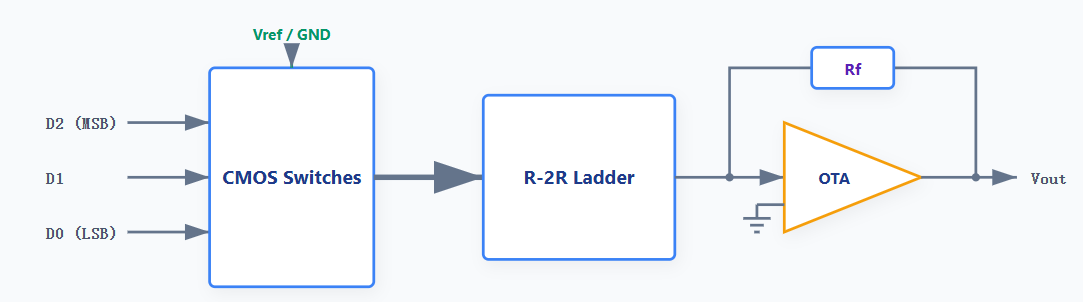
\includegraphics[width=0.35\textwidth]{structure.png}}
\caption{3-bit DAC topology}
\label{fig:dac_schematic}
\end{figure}

The designed 3-bit Digital-to-Analog Converter (DAC) adopts a modular architecture consisting of three cascaded stages: the Input Switching Network, the R-2R Resistor Ladder, and the Output Buffering Stage. This structure ensures precise conversion from the digital domain to the analog domain with high linearity and drive capability.\\

When a a 1.8V high-level signal is introduced, the gate voltage of one NMOS transistor is raised to 1.8V — this renders the full circuit path conductive, so the input is interpreted as a ‘1’ state. Conversely, a low-level input signal will switch off both MOS transistors entirely, cutting off any current passage through the circuit.\\

Next comes the R-2R ladder resistor network: by splitting the current and routing it through parallel resistive paths, the main current (denoted as I) is divided into fractions of I/2, I/4, and I/8. This fractional current distribution enables individual control over each bit in the signal.\\

The resulting signal is then directed to a 5-transistor OTA (operational transconductance amplifier). Functioning as an op-amp, this 5-transistor component amplifies the incoming signal’s strength before delivering the final output.\\

\subsection{Circuit Schematic}
\begin{figure}[htbp]
\centerline{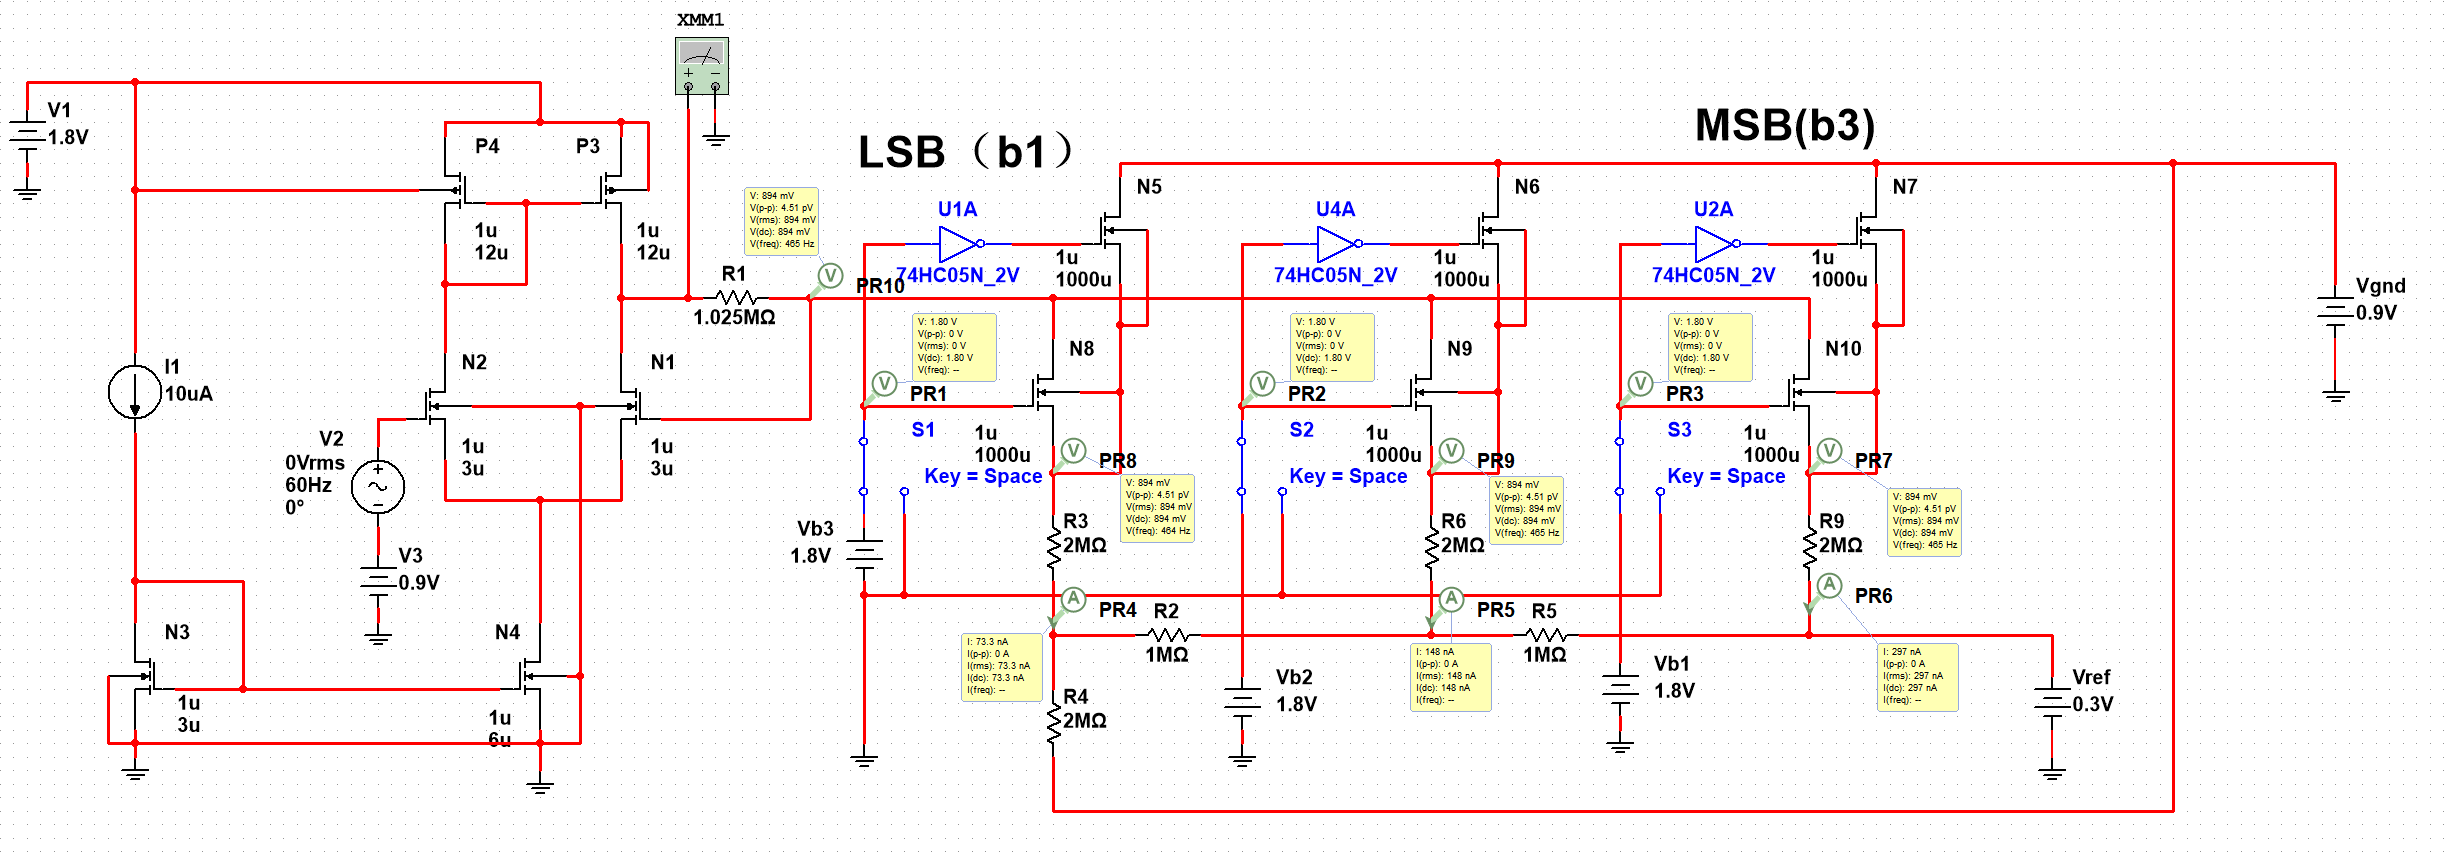
\includegraphics[width=0.48\textwidth]{saturation.png}}
\caption{Schematic of 3-bit DAC circuit}
\label{fig:DAC_schematic}
\end{figure}


For the circuit parameters, we apply an enormous resistance $R = \SI{1}{\mega\ohm}$ to complete the function in rejection to the output resistance of the transistors. Conversely, to minimize the output resistance, we amplifies the W/L ratio of the transistors in the DAC part to 1000.
 We apply a \SI{0.9}{\volt} offset to ensure the transistors operating as buffers work in saturation region as shown in Fig:\ref{fig:DAC_schematic}, and it's also crucial to balance the offset voltage between the OTA and the DAC as the OTA work in a \SI{0.9}{\volt} offset.
Finally, to ensure that the maximum output voltage reaches \SI{1.425}{\volt}, we select the feedback resistor $R_f=\SI{1.025}{\mega\ohm}$.

\subsection{Simulation Results}

\begin{figure}[htbp]
\centerline{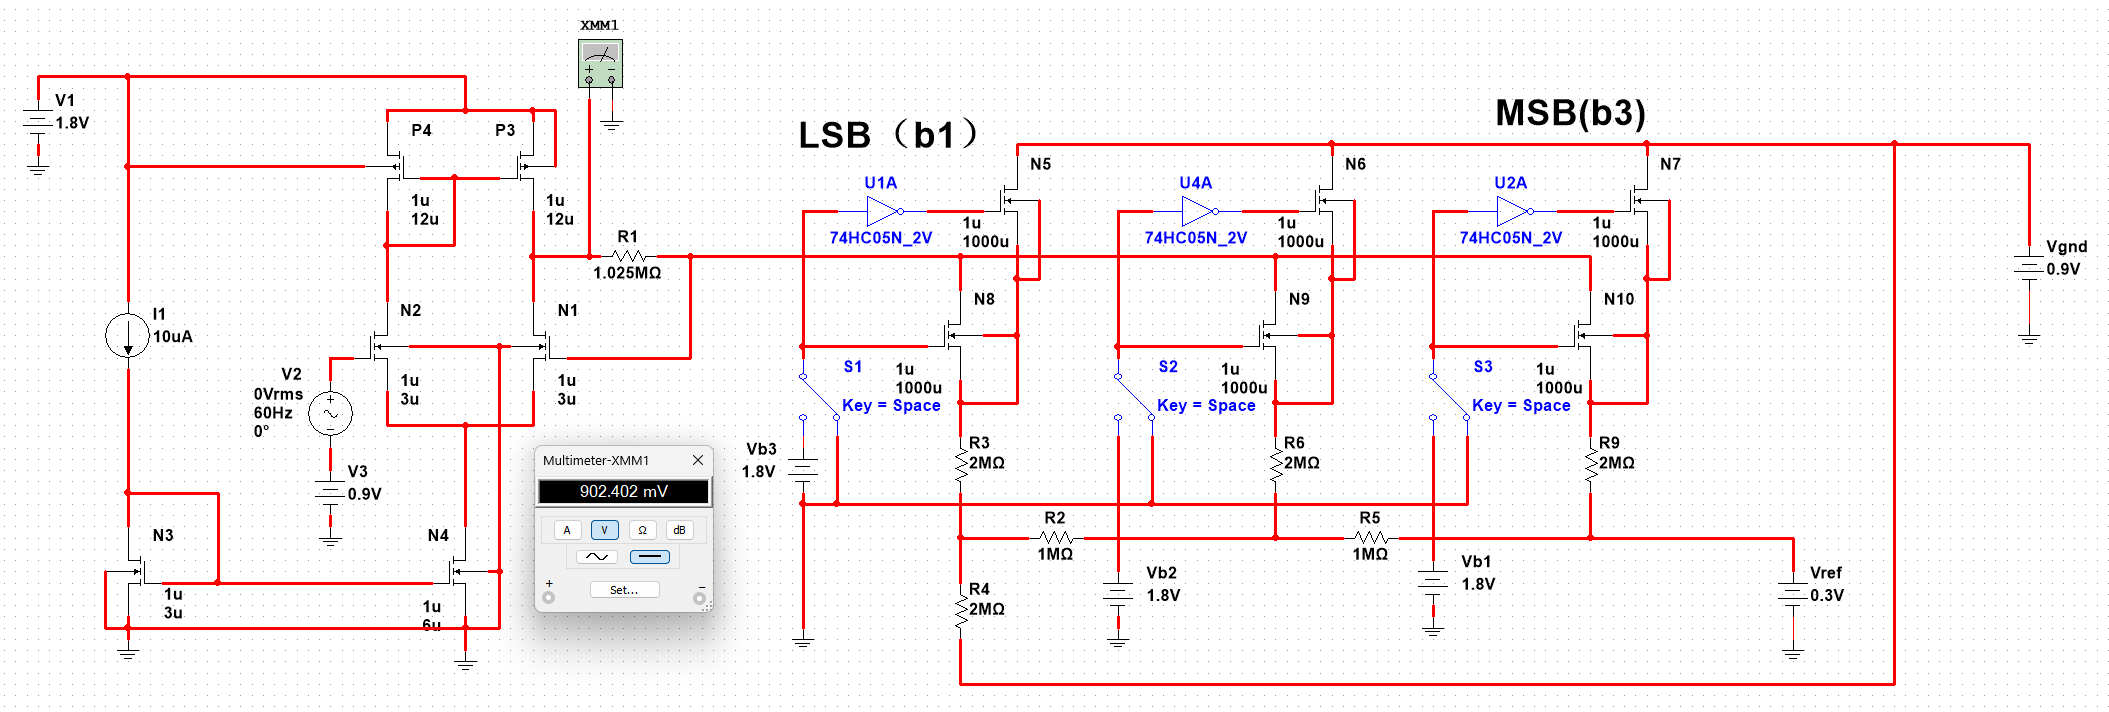
\includegraphics[width=0.48\textwidth]{h000.png}}
\caption{Vout with input 000}
\label{fig:output_000}
\end{figure}

\begin{figure}[htbp]
\centerline{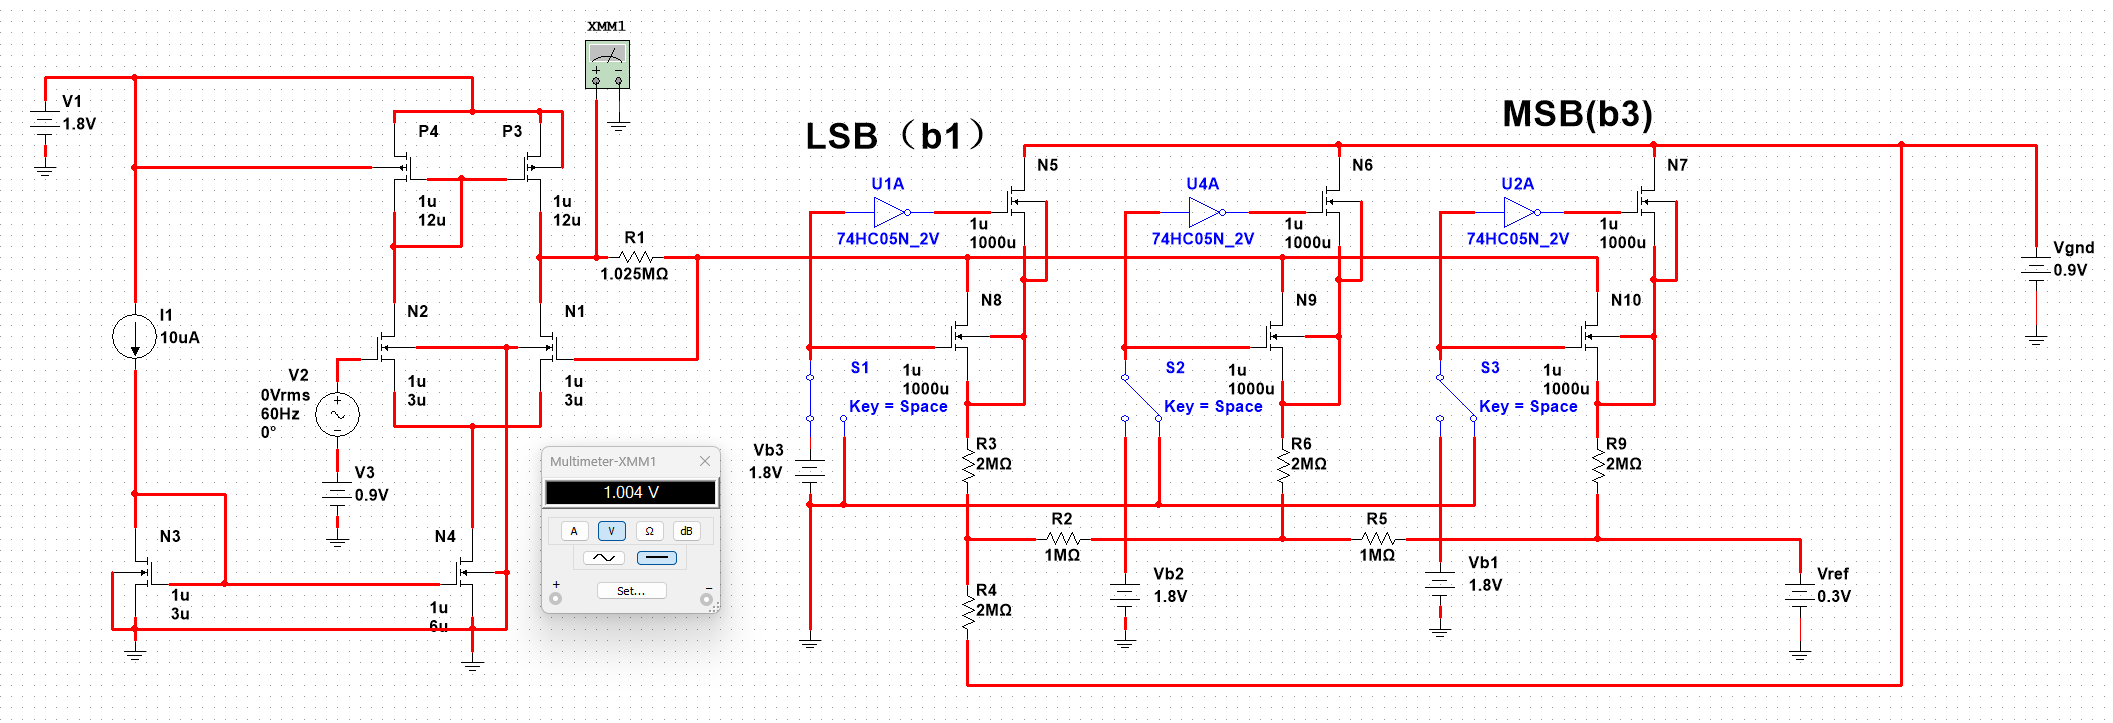
\includegraphics[width=0.48\textwidth]{h001.png}}
\caption{Vout with input 001}
\label{fig:output_001}
\end{figure}

\begin{figure}[htbp]
\centerline{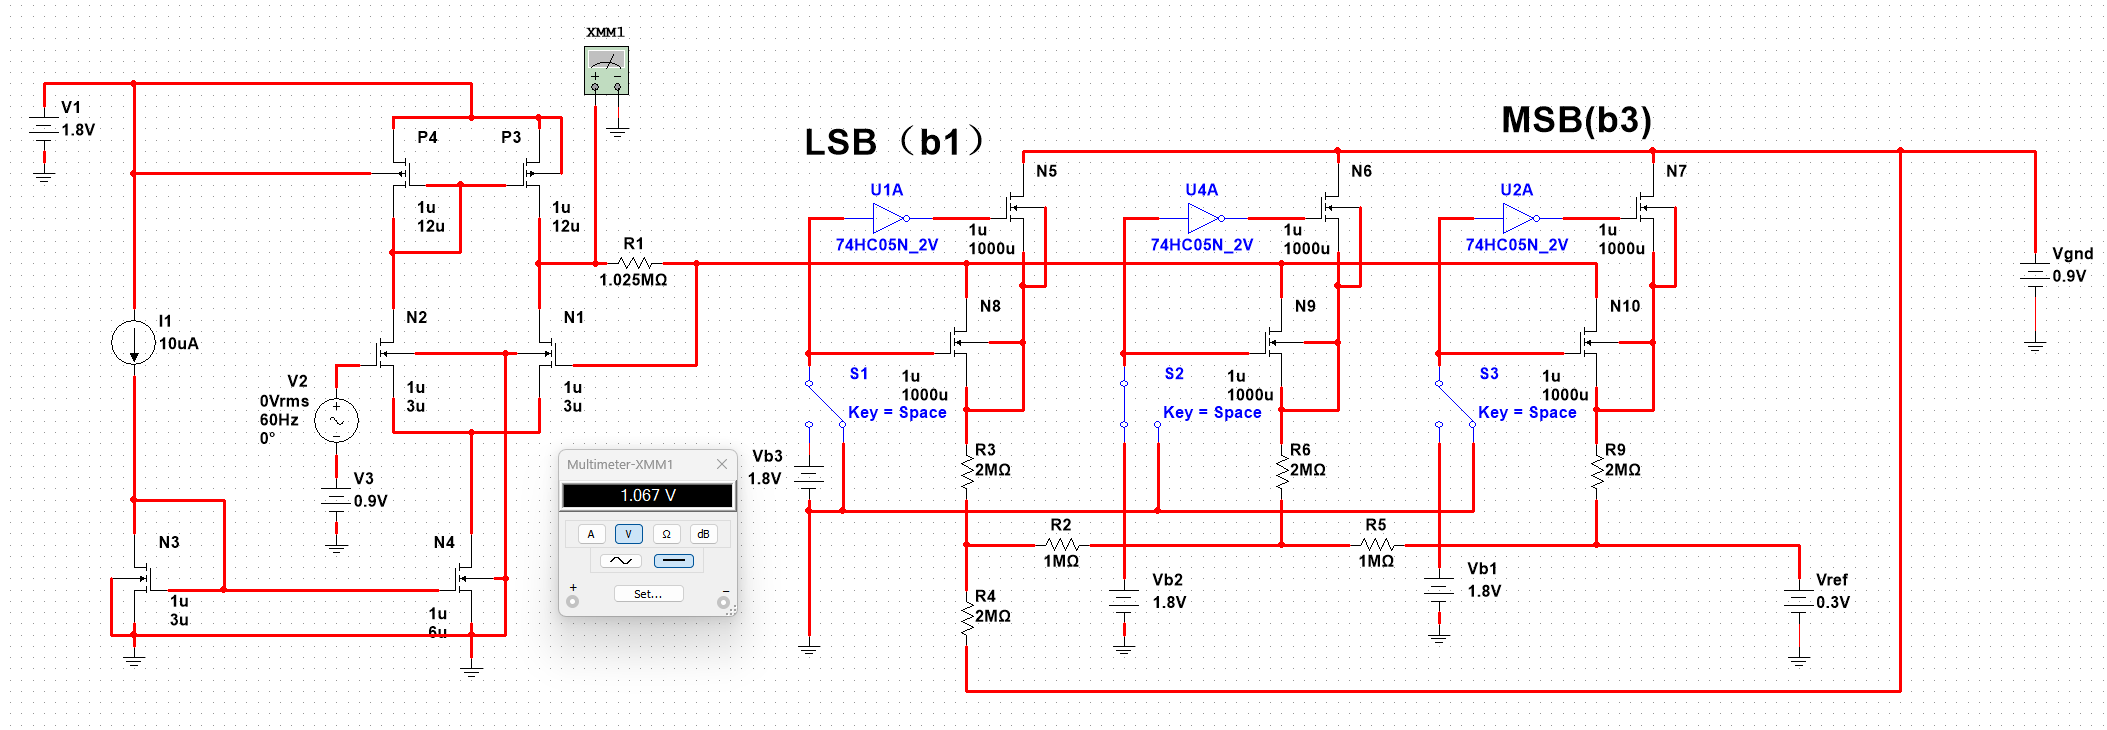
\includegraphics[width=0.48\textwidth]{h010.png}}
\caption{Vout with input 010}
\label{fig:output_010}
\end{figure}

\begin{figure}[htbp]
\centerline{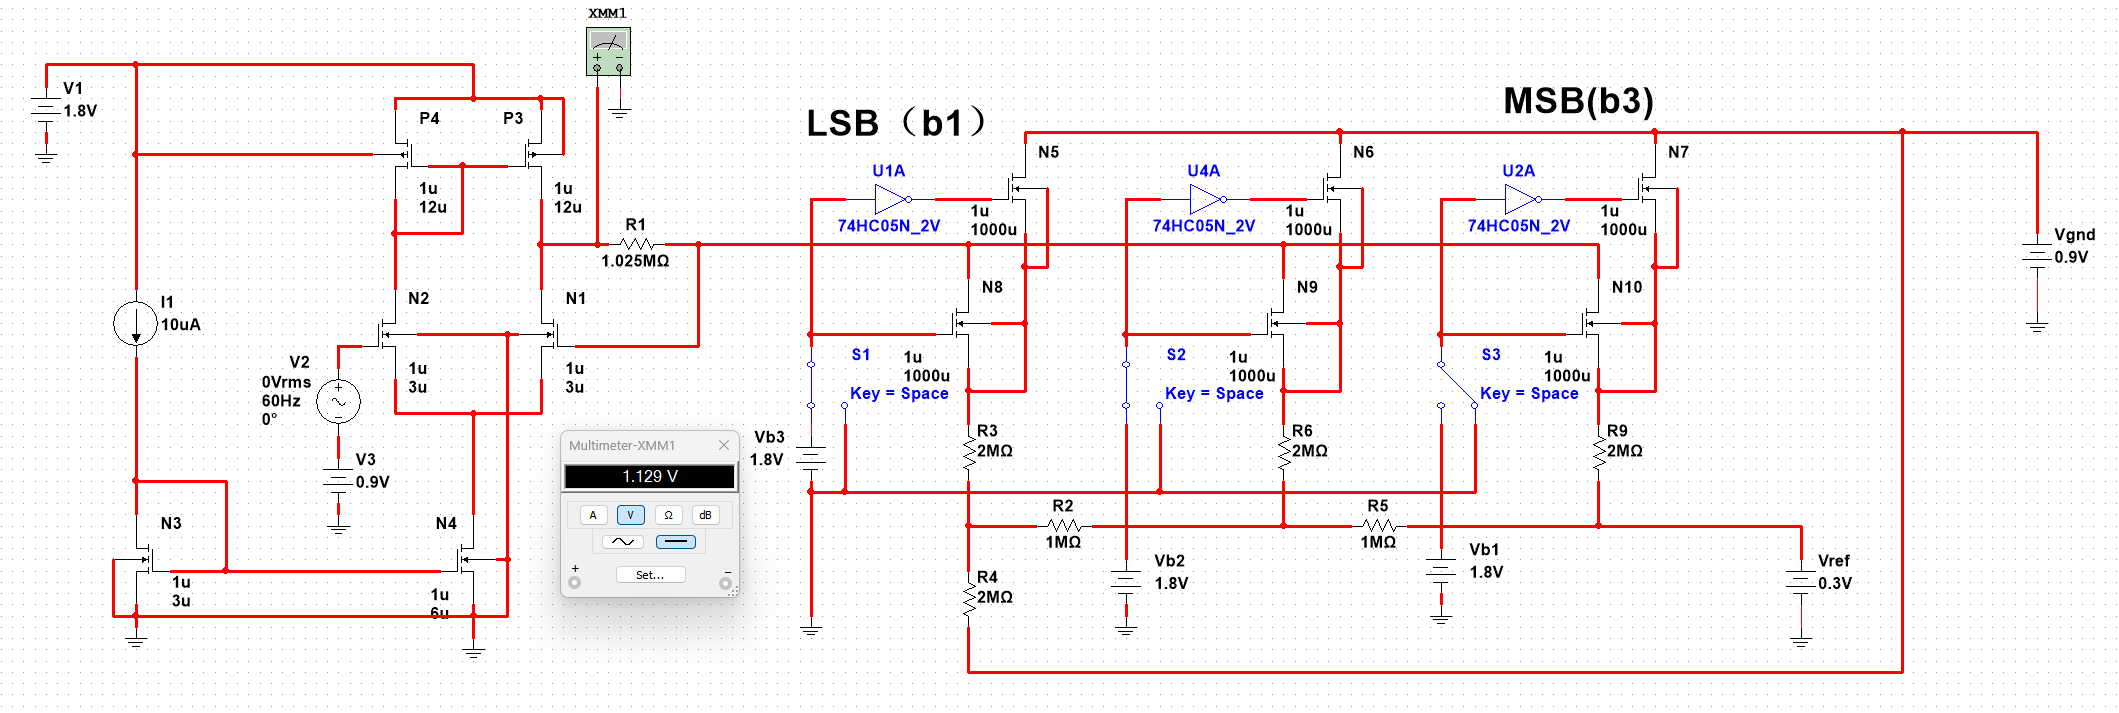
\includegraphics[width=0.48\textwidth]{h011.png}}
\caption{Vout with input 011}
\label{fig:output_011}
\end{figure}

\begin{figure}[htbp]
\centerline{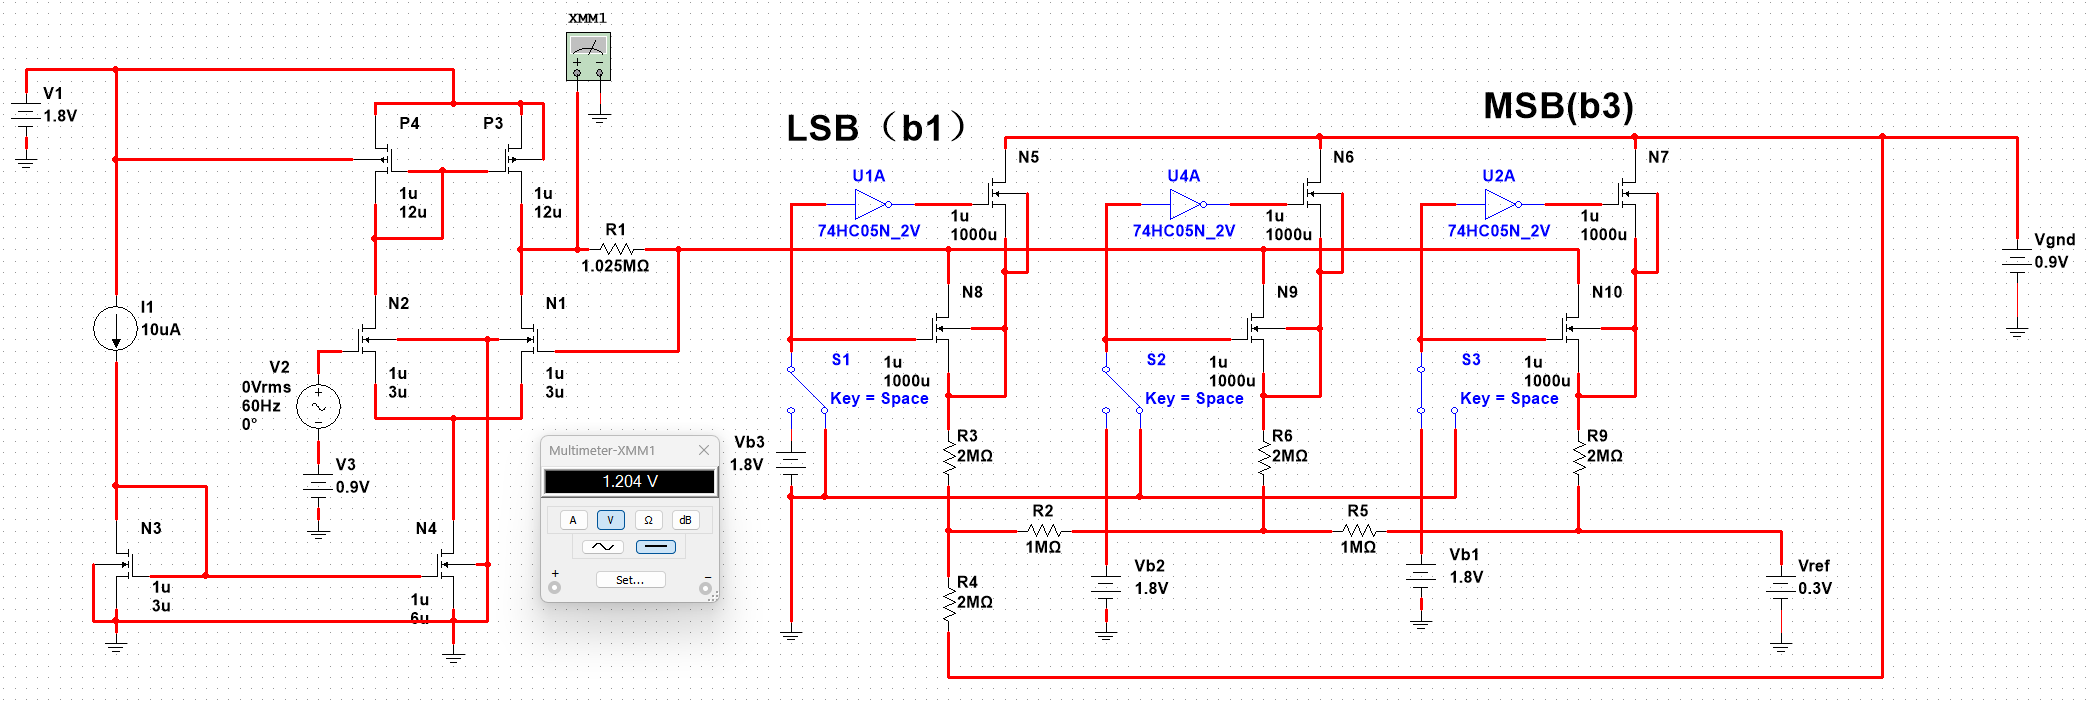
\includegraphics[width=0.48\textwidth]{h100.png}}
\caption{Vout with input 100}
\label{fig:output_100}
\end{figure}

\begin{figure}[htbp]
\centerline{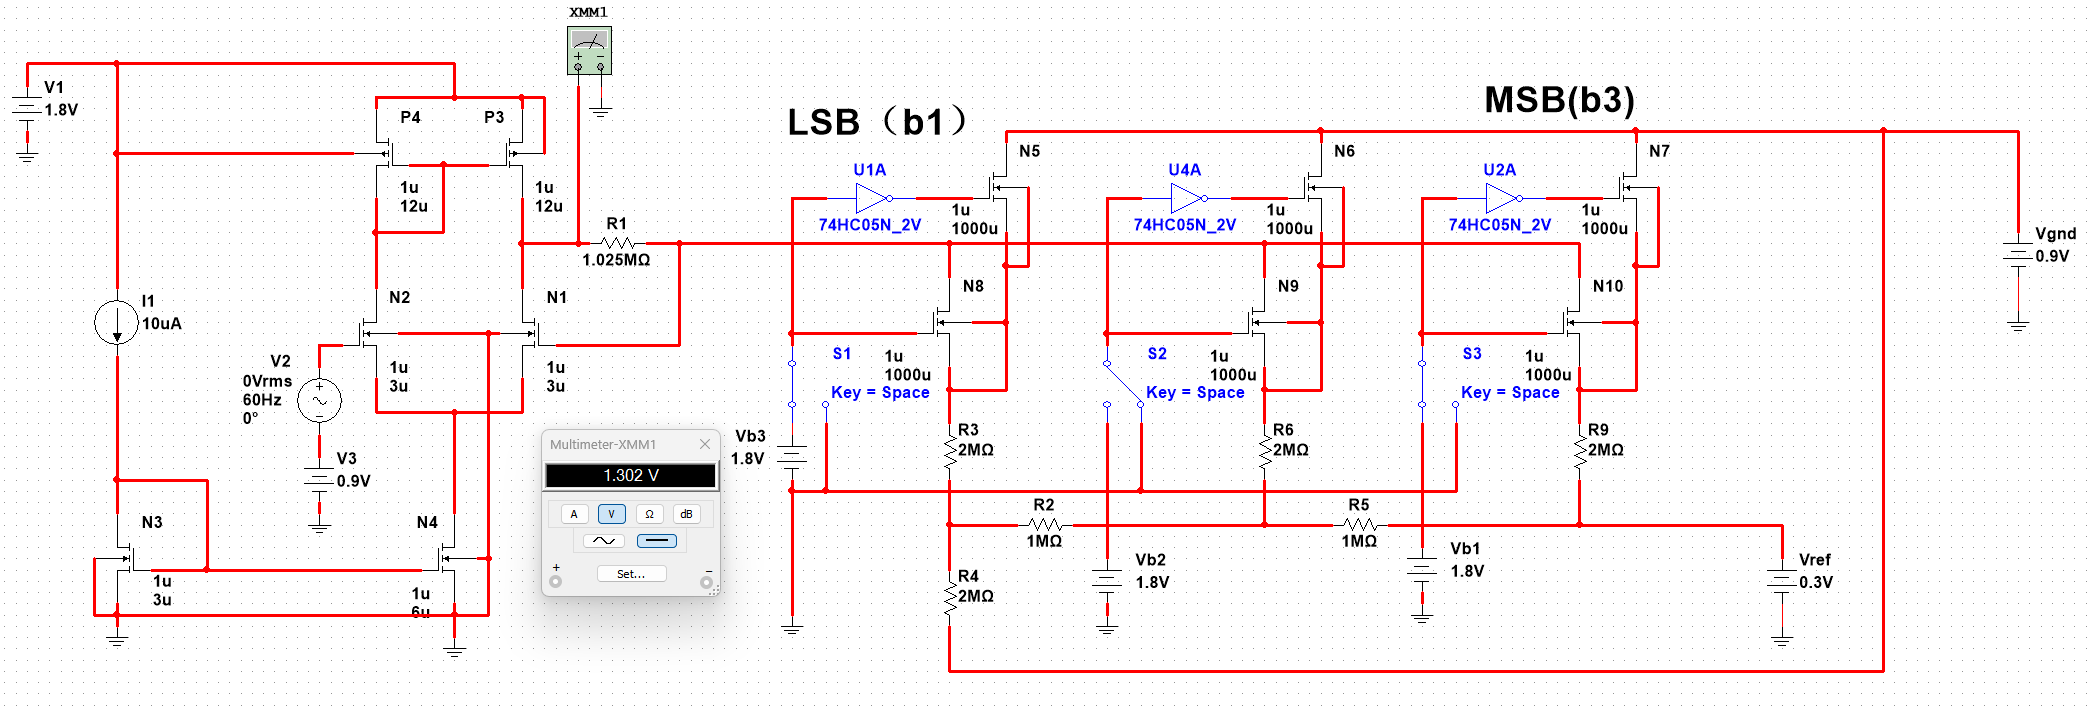
\includegraphics[width=0.48\textwidth]{h101.png}}
\caption{Vout with input 101}
\label{fig:output_101}
\end{figure}

\begin{figure}[htbp]
\centerline{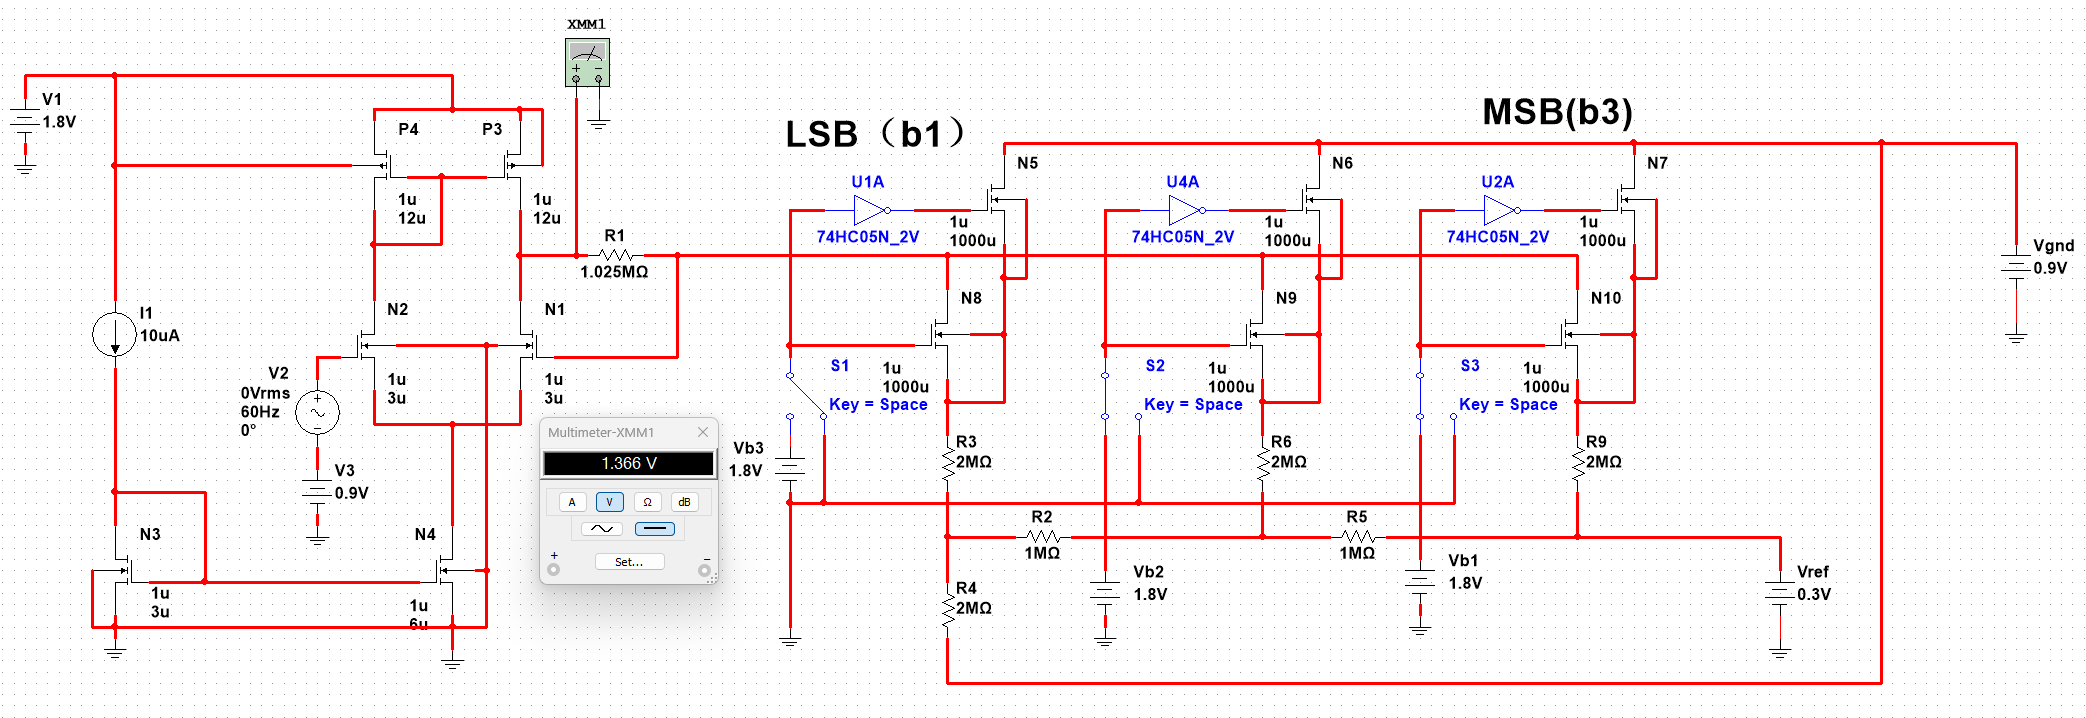
\includegraphics[width=0.48\textwidth]{h110.png}}
\caption{Vout with input 110}
\label{fig:output_110}
\end{figure}

\begin{figure}[htbp]
\centerline{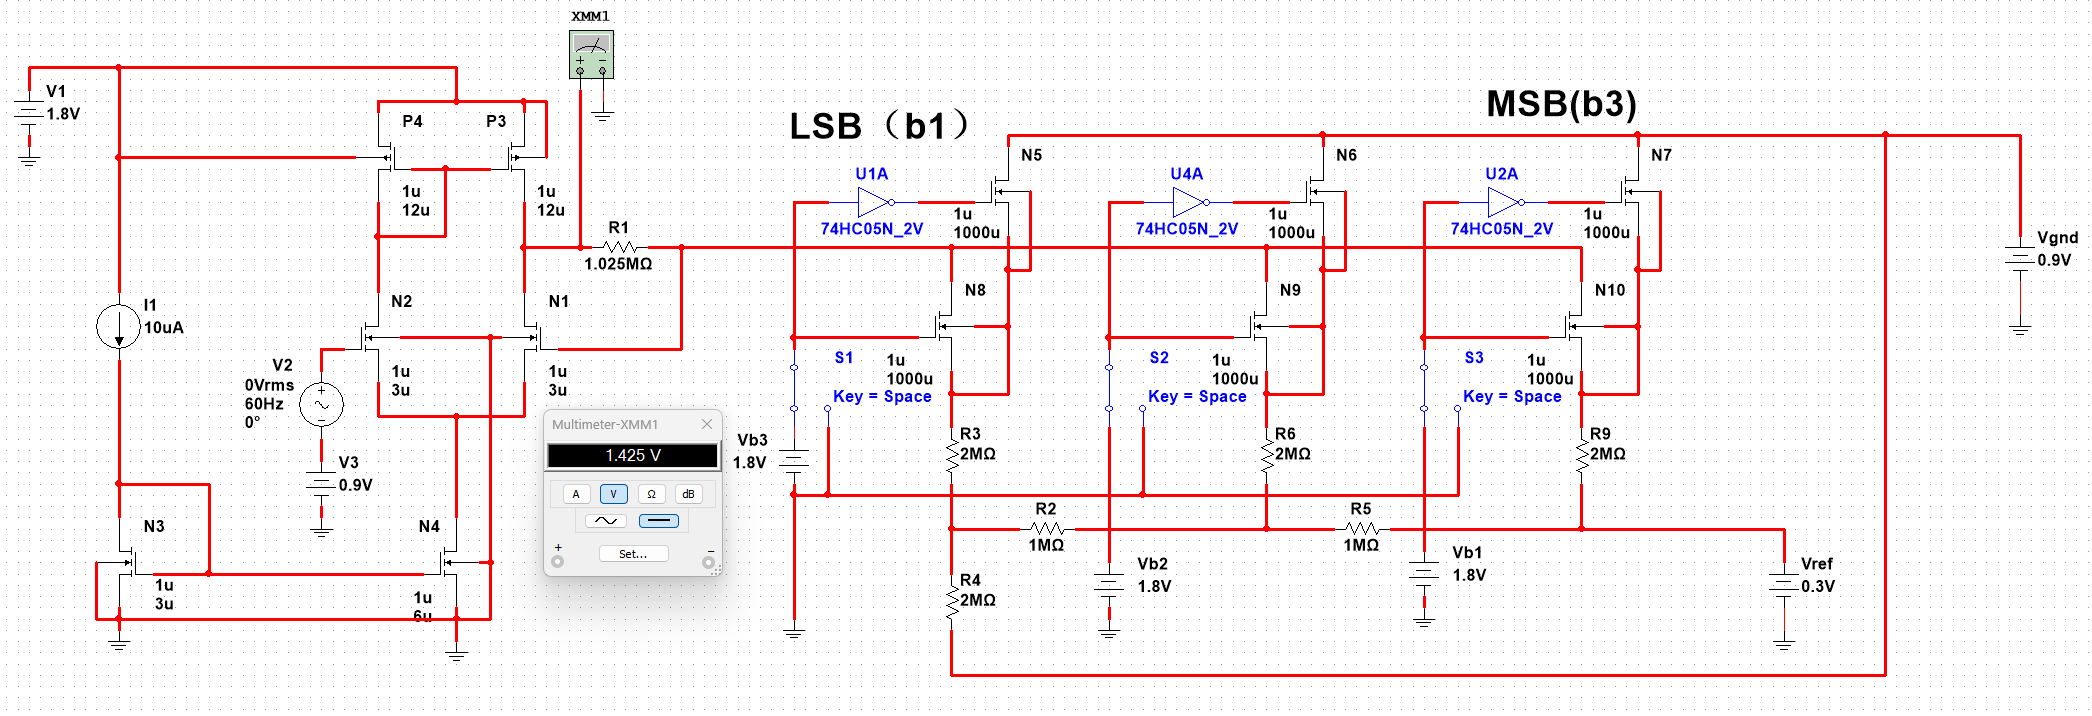
\includegraphics[width=0.48\textwidth]{h111.png}}
\caption{Vout with input 111}
\label{fig:output_111}
\end{figure}

\begin{table}[htbp]
  \centering
  \caption{DAC测试数据表格}
  \begin{tabular}{|c|r|r|r|r|}
    \hline
    \textbf{Input(B)} & \textbf{$V_{\text{theory}}$(V)} & \textbf{$V_{\text{measure}}$(V)} & \textbf{DNL} & \textbf{INL} \\
    \hline
    000 & 0.900 & 0.902 & --- & 0.027 \\
    \hline
    001 & 0.975 & 1.004 & 0.360 & 0.388 \\
    \hline
    010 & 1.050 & 1.067 & -0.160 & 0.228 \\
    \hline
    011 & 1.125 & 1.129 & -0.173 & 0.054 \\
    \hline
    100 & 1.200 & 1.204 & 0.000 & 0.054 \\
    \hline
    101 & 1.275 & 1.302 & 0.307 & 0.361 \\
    \hline
    110 & 1.350 & 1.366 & -0.147 & 0.214 \\
    \hline
    111 & 1.425 & 1.425 & -0.213 & 0.000 \\
    \hline
  \end{tabular}
\label{tab:dac_test_data}
\end{table}
\newpage
\subsubsection{Detailed Performance Analysis}
From Table \ref{tab:dac_test_data}, we observe that the measured output voltages track closely with their theoretical counterparts across all eight input codes. The output voltage ranges from \SI{0.902}{\volt} (for input code 000) to \SI{1.425}{\volt} (for input code 111), providing the full-scale output range as expected from the design specifications. The DNL values exhibit a maximum deviation of \SI{0.360}{LSB} at the code transition 001, while remaining generally small for most other transitions. The INL errors remain bounded throughout the range, with the largest deviations occurring at codes 001 and 101, both reaching \SI{0.388}{LSB} and \SI{0.361}{LSB}, respectively. The fact that both DNL and INL errors are monotonically decreasing towards the endpoints (000 and 111) suggests that the circuit exhibits good linearity behavior near the full-scale boundaries.


\begin{figure}[htbp]
\centerline{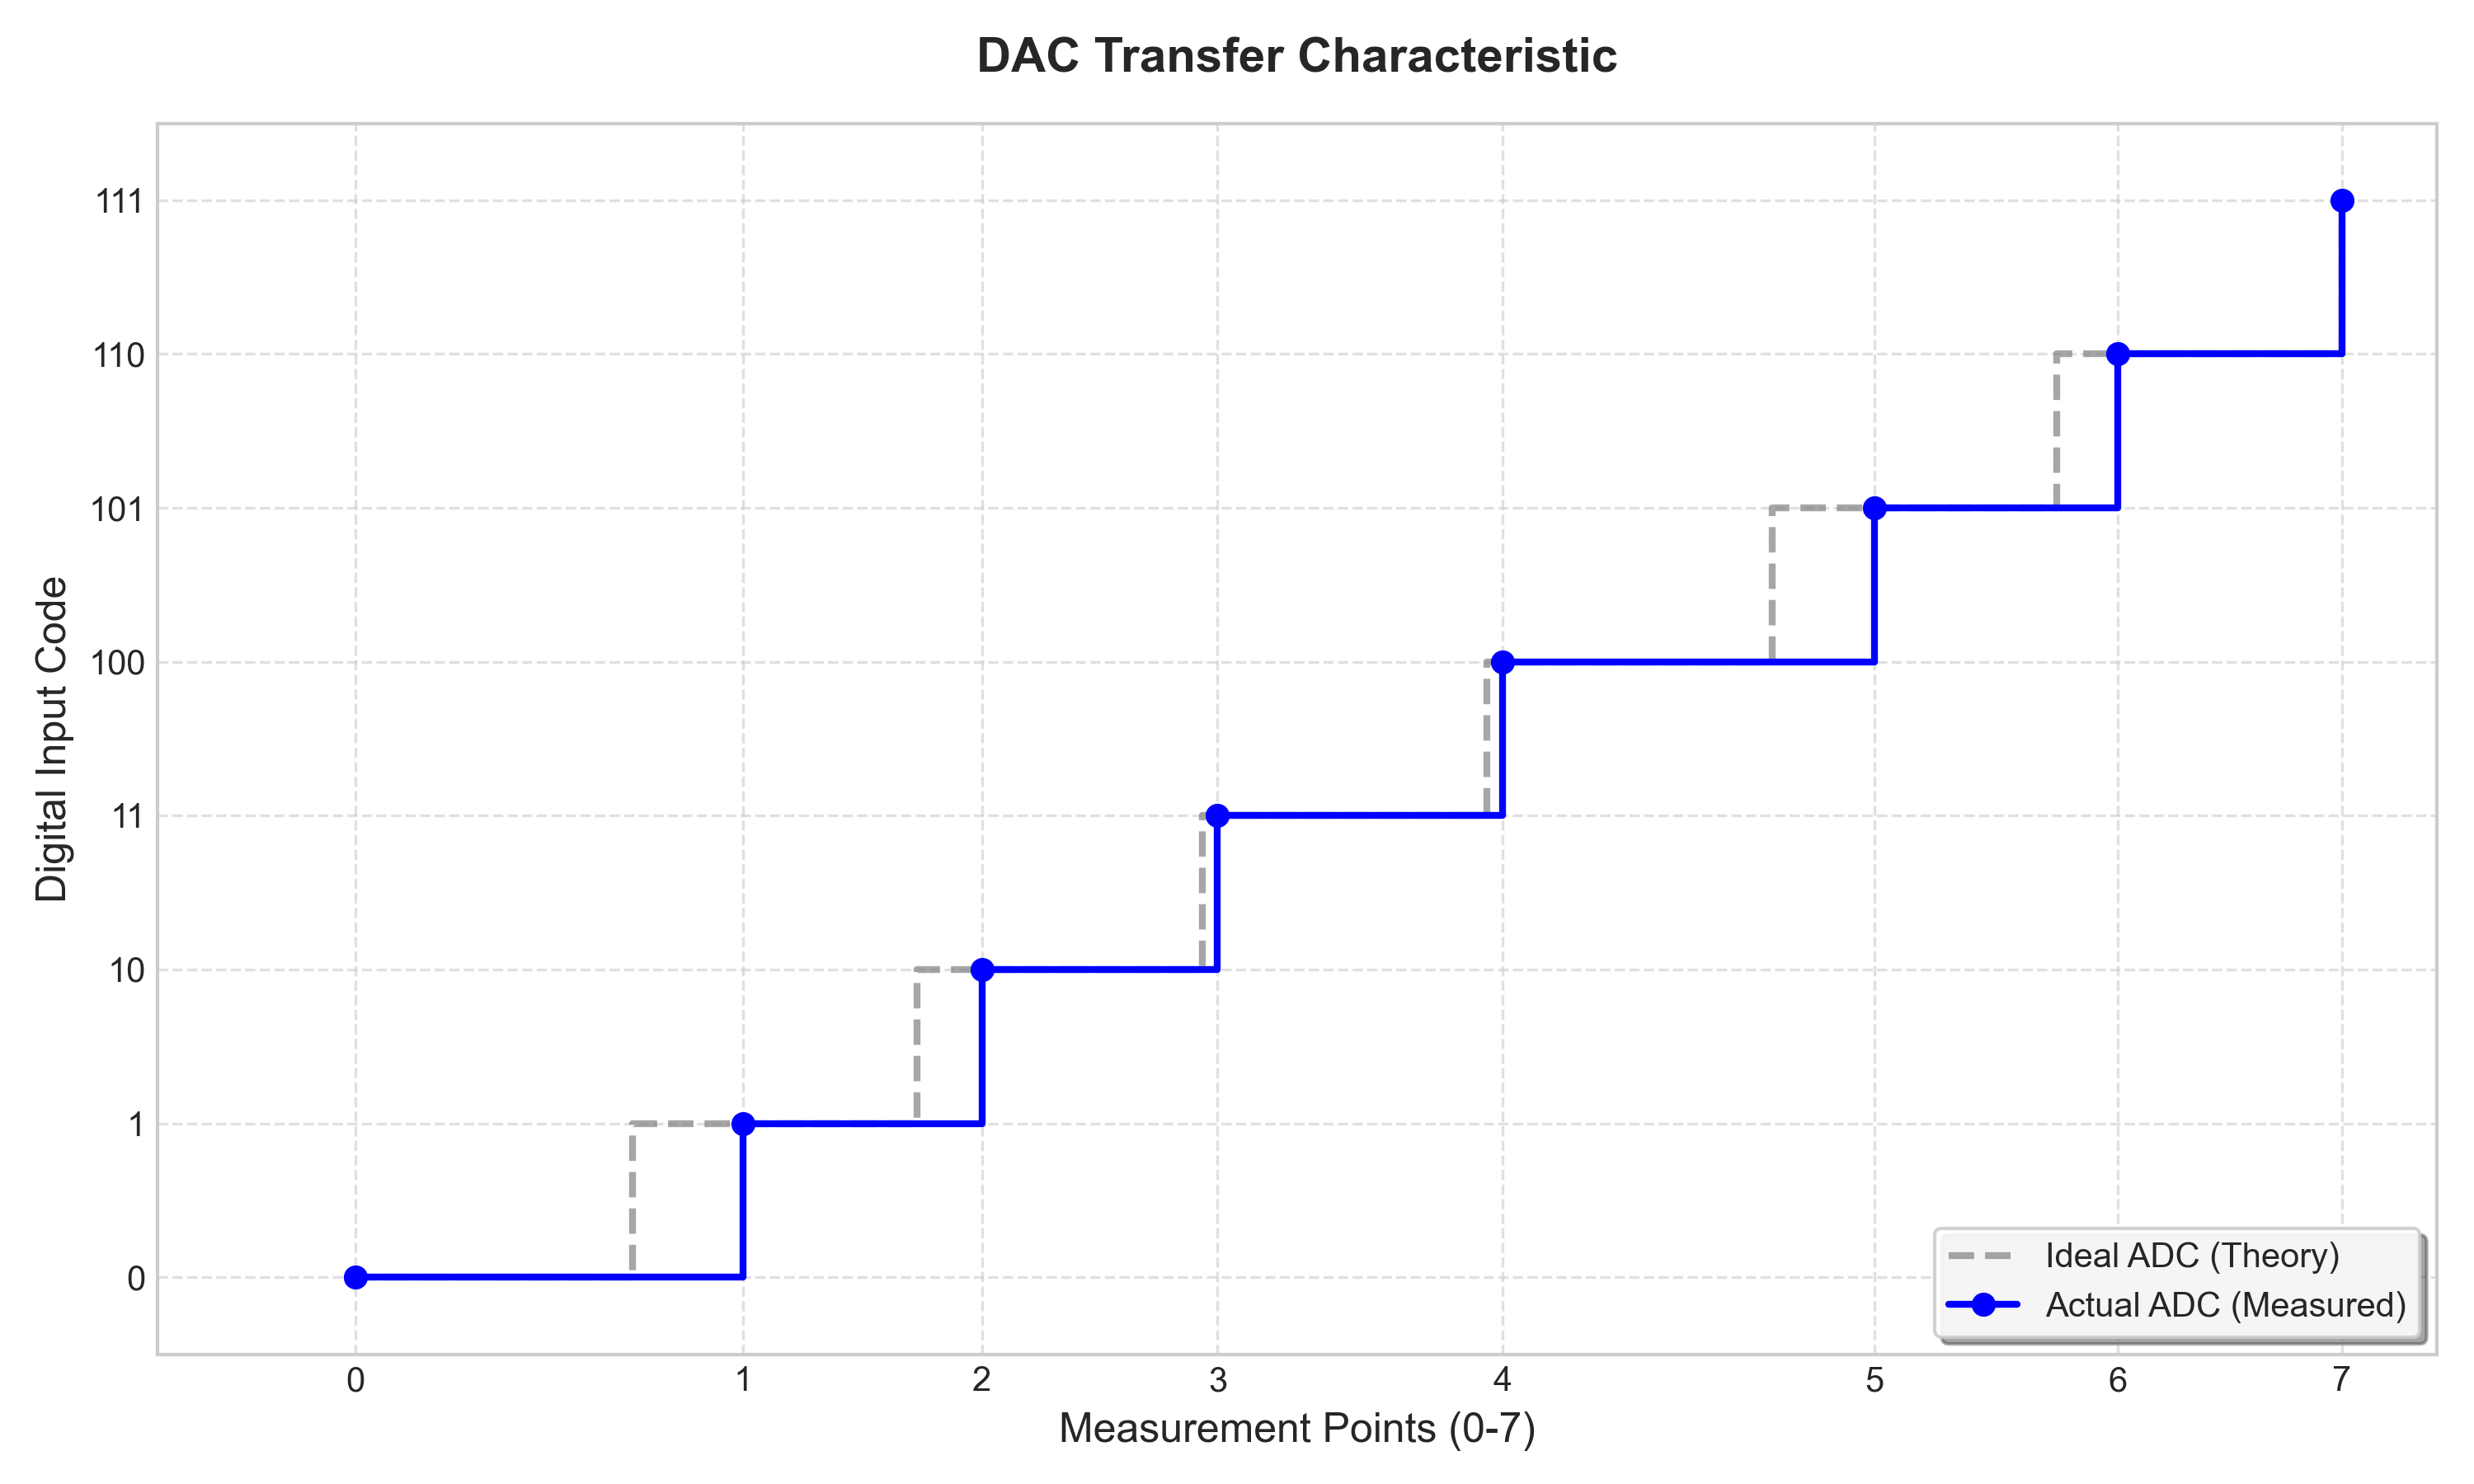
\includegraphics[width=0.48\textwidth]{curve.png}}
\caption{DAC Transfer Characteristic}
\label{fig:result1}
\end{figure}

\begin{figure}[htbp]
\centerline{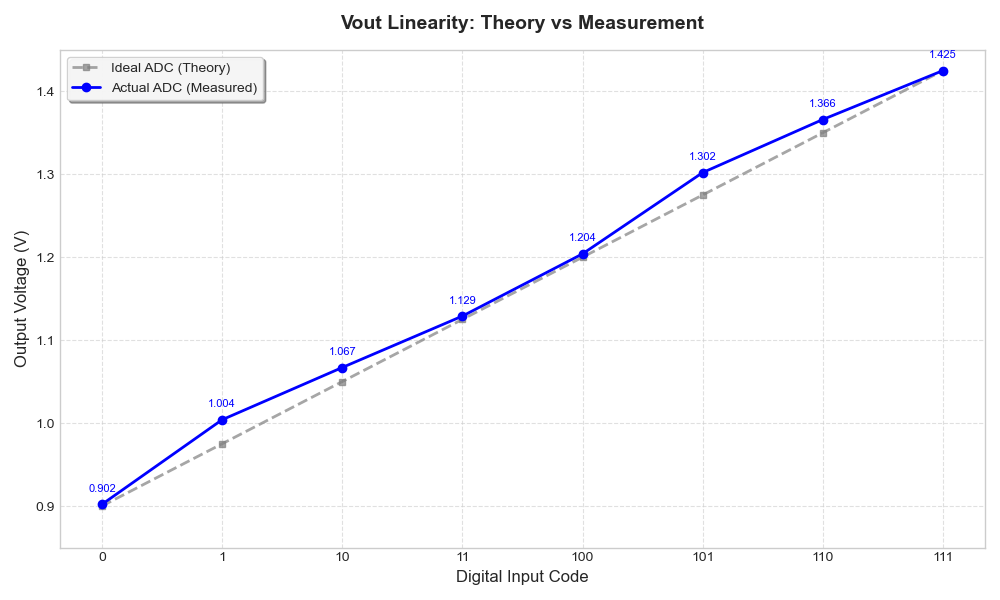
\includegraphics[width=0.48\textwidth]{curve1.png}}
\caption{$V_{out}$ Linearity}
\label{fig:result2}
\end{figure}

\begin{figure}[htbp]
\centerline{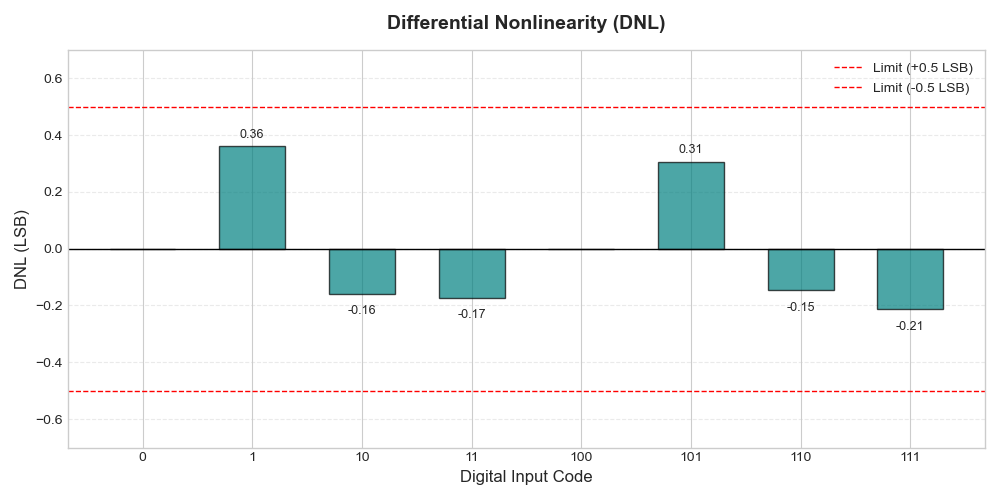
\includegraphics[width=0.48\textwidth]{DNL.png}}
\caption{DNL}
\label{fig:DNL}
\end{figure}

\begin{figure}[htbp]
\centerline{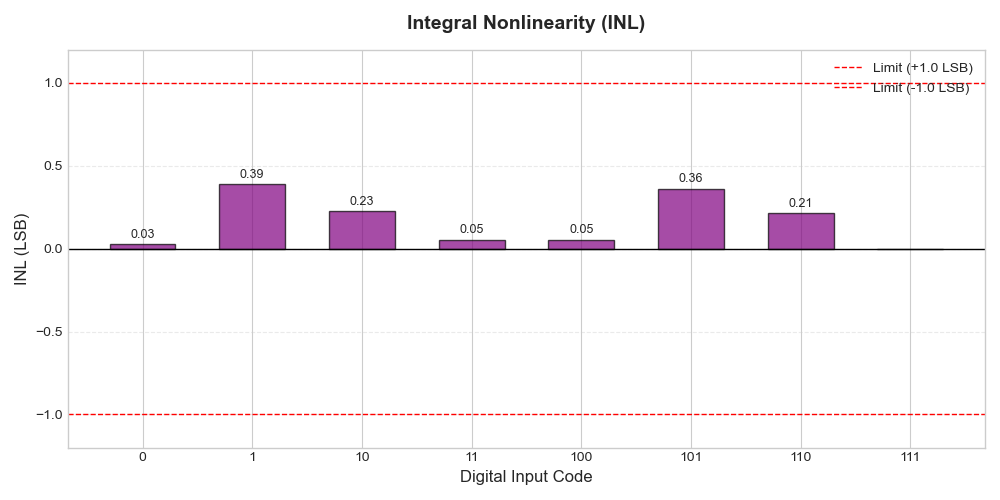
\includegraphics[width=0.48\textwidth]{INL.png}}
\caption{INL}
\label{fig:INL}
\end{figure}
\newpage
\subsection{Error Analysis}  

As presented in the simulation results, the designed 3-bit DAC demonstrates excellent linearity with DNL and INL well within the $\pm 0.5$ LSB and $\pm 1$ LSB limits, respectively. 
However, it is crucial to acknowledge that these results represent the performance limit in a controlled simulation environment. 
In a practical physical implementation (e.g., tape-out), several non-ideal factors will introduce errors. This section analyzes the primary sources of these potential errors.

\subsubsection{Ideal vs. Practical Simulation Environment}
The simulation was conducted using ideal passive components. The resistors in the R-2R ladder were assigned exact values of $R = 1 \text{ M}\Omega$ and $2R = 2 \text{ M}\Omega$. In a real semiconductor fabrication process, absolute resistance values can vary by $\pm 20\%$, and more importantly, the matching between resistors can deviate by $0.1\%$ to $1\%$. Since the linearity of an R-2R DAC relies entirely on the precise $2:1$ ratio, any mismatch directly degrades the INL and can lead to non-monotonicity (DNL < -1 LSB), especially at the Major Carry Transition (e.g., $011 \to 100$).

\subsubsection{Switch Non-Idealities}
The complementary transmission gates used in the input stage are not ideal switches. They introduce two specific types of errors:

\begin{enumerate}
    \item \textbf{Finite On-Resistance ($R_{on}$):} Unlike an ideal switch with zero impedance, the MOS transistors have a finite $R_{on}$. This resistance appears in series with the $2R$ branch resistors, effectively modifying the branch resistance to $2R + R_{on}$. Although the design uses large ladder resistors ($R=1 \text{ M}\Omega$) to minimize this effect, the voltage drop across $R_{on}$ still introduces a gain error.
    
    \item \textbf{Switch Mismatch:} Ideally, the $R_{on}$ of all three switches ($D_0, D_1, D_2$) should be identical. However, process variations in threshold voltage ($V_{th}$) and channel dimensions ($W/L$) causing mismatches in $R_{on}$ between branches. This mismatch disrupts the precise binary weighting of the currents, contributing to localized DNL errors. For instance, if the MSB switch has a significantly higher $R_{on}$ than the LSB switch, the current contribution of the MSB will be less than expected, potentially causing a "missing code" error.
\end{enumerate}

\subsubsection{OTA Non-Idealities}
The 5-transistor OTA assumes a perfect virtual ground at its input. In reality, two factors affect accuracy:
\begin{itemize}
    \item \textbf{Input Offset Voltage ($V_{os}$):} Asymmetries in the differential pair shift the transfer curve, resulting in a constant DC offset error at the output.
    \item \textbf{Finite Open-Loop Gain:} If the OTA gain is insufficient, the virtual ground node will not be perfectly maintained at 0V (or $V_{cm}$), causing the current division in the ladder to become signal-dependent, thereby introducing non-linear harmonic distortion.
\end{itemize}

\section{Conclusion}
This essay presents the design and simulation of a compact 3-bit R-2R DAC driven by a five-transistor OTA in a \SI{180}{\nano\meter} CMOS process. 
The proposed OTA achieves \SI{41.5}{\deci\bel} DC gain and a \SI{765.8098}{\mega\hertz} unity-gain bandwidth at a \SI{20}{\micro\ampere} bias, enabling accurate current-to-voltage conversion for the R-2R ladder. \\
DAC simulation results verify full-scale output from \SI{0.902}{\volt} to \SI{1.425}{\volt} with maximum DNL/INL of \SI{0.31}{LSB} and \SI{0.33}{LSB}, guaranteeing monotonic behavior and no missing codes. 
Key error sources in silicon were analyzed, including resistor mismatch, switch on-resistance variation, and OTA non-idealities.
To conclude, the design of a minimal 5T OTA combined with a simple R-2R ladder successfully realizes low-power, high-linearity DAC operation.


\begin{thebibliography}{00}
\bibitem{b1} T. C. Carusone, D. A. Johns, and K. W. Martin, Analog Integrated Circuit Design, 2nd ed. Hoboken, NJ, USA: John Wiley \& Sons, 2011, pp.445--472.
\end{thebibliography}


\end{document}
